\documentclass[acmlarge]{acmart}
\usepackage[
    type={CC},           % your choice
    modifier={by-sa},    % your choice
    version={4.0},       % your choice
]{doclicense}  

\settopmatter{printacmref=false}
\fancyfoot{}

\makeatletter
\def\@formatdoi#1{}
\def\@permissionCodeOne{miniKanren.org/workshop}
\def\@copyrightpermission{\doclicenseThis} 
\def\@copyrightowner{Copyright held by the author(s).}
\makeatother

\copyrightyear{2020}
\setcopyright{rightsretained}

\acmMonth{8}
\acmArticle{3}


\usepackage{listings}
\usepackage[section]{placeins}
\usepackage{multirow}
\usepackage{pgfplots}
\usepackage{yfonts}
\usepackage{subcaption}
\usepackage{xspace}

\pgfplotsset{width=7cm,compat=1.8}

\lstdefinelanguage{ocanren}{
keywords={run, conde, fresh, let, in, match, with, when, class, type,
object, method, of, rec, until, while, not, do, done, as, val, inherit,
new, module, sig, deriving, datatype, struct, if, then, else, open, private, virtual, include, success, failure,
true, false},
sensitive=true,
commentstyle=\small\itshape\ttfamily,
keywordstyle=\textbf,%\ttfamily\underline,
identifierstyle=\ttfamily,
basewidth={0.5em,0.5em},
columns=fixed,
mathescape=true,
fontadjust=true,
literate={fun}{{$\lambda$}}1 {->}{{$\to$}}3 {===}{{$\equiv$}}1 {=/=}{{$\not\equiv$}}1 {|>}{{$\triangleright$}}3 {\\/}{{$\vee$}}2 {/\\}{{$\wedge$}}2 {^}{{$\uparrow$}}1,
morecomment=[s]{(*}{*)}
}

\lstset{
language=ocanren
}

\newcommand{\ruleno}[1]{\mbox{[\textsc{#1}]}}
\newcommand{\rulen}[1]{[\textsc{#1}]}
\newcommand{\mk}{\textsc{miniKanren}\xspace}
\newcommand{\inbr}[1]{\langle #1 \rangle}

\let\oldemptyset\emptyset
\let\emptyset\varnothing

\begin{document}

\title{On Fair Relational Conjunction}

\author{Petr Lozov}
\email{lozov.peter@gmail.com}        

\author{Dmitry Boulytchev}
\email{dboulytchev@math.spbu.ru}    

\affiliation{
  \institution{Saint Petersburg State University}
  \country{Russia}                   
}

\affiliation{
  \institution{JetBrains Research}   
  \country{Russia}                   
}

\begin{abstract}
We present a new, more symmetric evaluation strategy for conjunctions in \mk. Unlike the original unfair directed conjunction, our approach controls the order of conjunct execution based on the properties of structurally recursive relations. In this paper we describe operational semantics for both ``classical'' and ``fair'' conjunctions. We also compare the performance of classical and fair conjunctions on a number of examples and discuss the results of the evaluation.
\end{abstract}

\begin{CCSXML}
<ccs2012>
   <concept>
       <concept_id>10011007.10011006.10011008.10011009.10011015</concept_id>
       <concept_desc>Software and its engineering~Constraint and logic languages</concept_desc>
       <concept_significance>500</concept_significance>
       </concept>
   <concept>
       <concept_id>10011007.10011006.10011039.10011311</concept_id>
       <concept_desc>Software and its engineering~Semantics</concept_desc>
       <concept_significance>500</concept_significance>
       </concept>
 </ccs2012>
\end{CCSXML}

\ccsdesc[500]{Software and its engineering~Constraint and logic languages}
\ccsdesc[500]{Software and its engineering~Semantics}

\keywords{relational programming, miniKanren, evaluation strategies, operational semantics}

\maketitle

\thispagestyle{empty}

\section{Introduction}
\label{sec:intro}

Algebraic data types (ADT) is an important tool in functional programming which delivers a way to represent flexible and easy to manipulate data structures.
To inspect the contents of ADT values a generic construct~--- \emph{pattern matching}~--- is used. Pattern matching can be considered as a generalization of
conventional conditional control-flow construct ``\lstinline|if .. then .. else|'' and in principle can be decomposed into a nested hierarchy of those; from
this standpoint the problem of pattern matching implementation can be considered trivial. However, some decompositions are obviously better than others. We
repeat here an example from~\cite{maranget2008} to demonstrate this difference (see Fig.~\ref{fig:match-example}). Here we match a triple of boolean
values $x$, $y$, and $z$ against four pattern (Fig.~\ref{fig:matching-example1}; we use \textsc{OCaml}~\cite{ocaml} as reference language). The na\"{i}ve
implementation of this example is shown on Fig.~\ref{fig:matching-example2}; however if we decide to match $y$ first the result becomes much
better (Fig.~\ref{fig:matching-example3}).

\begin{figure}[ht]
\begin{subfigure}[t]{0.2\linewidth}
\centering
\begin{lstlisting}
match x, y, z with
| _, F, T -> 1
| F, T, _ -> 2
| _, _, F -> 3
| _, _, T -> 4
\end{lstlisting}
\vskip18.5mm
\caption{Pattern matching}
\label{fig:matching-example1}
\end{subfigure}
\hspace{0.5cm}
\begin{subfigure}[t]{0.26\linewidth}
\centering
\begin{lstlisting}
if x then
  if y then
    if z then 4 else 3
  else
    if z then 1 else 3
else
  if y then 2
  else
    if z then 1 else 3
\end{lstlisting}
\caption{A correct but non-optimal\\\phantom{(b)~}implementation}
\label{fig:matching-example2}
\end{subfigure}
\hspace{0.5cm}
\begin{subfigure}[t]{0.33\linewidth}
\centering
\begin{lstlisting}
if y then
  if x then
    if z then 4 else 3
  else 2
else
  if z then 1 else 3
\end{lstlisting}
\vskip13.5mm
\caption{Optimal implementation}
\label{fig:matching-example3}
\end{subfigure}
\caption{Pattern matching implementation example} 
\label{fig:match-example}
\end{figure}

\begin{comment}
\begin{figure}[ht]
\begin{minipage}[b]{0.3\linewidth}
\centering
\label{fig:figure1}
\end{minipage}
\hspace{0.5cm}
\begin{minipage}[b]{0.3\linewidth}
\centering
\begin{lstlisting}
switch x with 
| true -> 
    switch y with 
    | true -> 
       switch z with 
       | true -> 4
       | _ -> 3
    | _ -> 
      switch z with 
      | true -> 1
      | _ -> 3 
| _ -> 
   switch y with 
   | true -> 2 
   | _ -> if z then 1 else 3
\end{lstlisting}
\end{minipage}
\hspace{0.5cm}
\begin{minipage}[b]{0.3\linewidth}
\centering
\end{minipage}
\end{figure}
\end{comment}


%clasification 1
Although semantics of pattern matching can be given as a sequence of srutinee's sub expression comparisons (Figure~\ref{fig:matchpatts}) effective compilers don't follow
this approach. One can either optimise runtime cost by minimizing amount of checks performed or static cost by minimizing the size of generated code. \emph{Decision trees}~\cite{?}
are good for the first criteria, because they check every subexpression not more than once. \emph{Backtracking automata} are rather compact but in some cases can perform
repeated checks.

%clasification 2
\emph{For strict languages} checking sub-expressions of scrutinee in any order is allowed. \emph{For lazy languages} pattern matching should evaluate only those sub-expressions which are
necessary for performing pattern matching. If not careful pattern matching can change the termination behavior of the program. In general lazy languages setup more constraints on pattern matching and because of that allow lesser set of heuristics. Decision trees and backtracking automata can be used for compilation both  strict and lazy languages.

%clasification 3
The matching compilers for strict languages can work in \emph{direct} or \emph{indirect} styles. The first ones return efficient code immediately. In the second style to
construct final answer some post processing is required. It can vary from easy simplifications to complicated supercompilation techniques~\cite{sestoft1996}. The main
drawback of indirect style is that the size of intermediate data structures can be exponentially large.

% about lazy languages
A few approaches for checking sub-expressions in lazy languages has been proposed. In ~\cite{augustsson1985} simple left-to-right order of subexpression checking was proposed and was proved that it doesn't affect termination. The backtracking automaton being built has a form of a DAG to reduce code size. A few refinements has been added by~\cite{wadler1987} as a part of textbook~\cite{peytonjones1987} about implementing lazy functional languages. The implementation from this book is being used in the current version of GHC~\cite{ghc}. \cite{laville1991} models values in lazy languages
using \emph{partial terms}, although it doesn't scale to types with infinite constructor sets (like integers). The approach doesn't test all subexpressions from left to right as~\cite{augustsson1985} but aims to not perform unnecessary check by constructing \emph{lazy automaton}. 
%In~\cite{suarez1993} the similar approach is extended by special treatment of overlapping patterns.

% about decision trees
Pattern matching for lazy languages has been compiled also to decision trees~\cite{maranget1992} and later (\cite{maranget1994}) into
\emph{decision DAGs} which allow in some cases to make code smaller.

Minimizing the size of decision tree is known to be NP-hard~\cite{baudinet1985tree}, and as a rule various heuristics are applied during compilation, for example, the number of nodes,
the length of the longest path, the average length of all paths. The paper~\cite{Scott2000WhenDM} performs experimental evaluation of nine heuristics on the base of for strict language Standard ML of New Jersey.

%about automata
The inefficiency of backtracking automaton has been
improved in~\cite{maranget2001}. The approach utilizes matrix representation for pattern matching. It splits the current matrix according to constructors in the
first column and reduces the task to compiling matrices with less rows. The technique is indirect, in the end a few optimizations are performed by introducing
special \emph{exit} nodes to the compiled representation. No preprocessing is required for this scheme: or-pattern receives a special treatment during compilation process.
The approach from this paper is used in the current implementation of the \textsc{OCaml} compiler.

Previous approach uses first column to split the matrix. In~\cite{maranget2008} the \emph{necessity} heuristic has been introduced which recommends which column should be
used to perform the split. Good decision trees which are constructed in this work can perform better on corner cases than~\cite{maranget2001}, but for practical cases the
difference is insignificant.


While existing approaches deliver appropriate solutions for certain forms of pattern matching construct, they have to be extended in an \emph{ad hoc} manner each time
the syntax and semantics of pattern matching construct changes. For example, besides a simple conventional form of pattern matching there is a number of extensions
(guards~\cite{?}, disjunctive patterns~\cite{?}, non-linear patterns~\cite{mcbride1969symbol}, active patterns~\cite{activepatterns}, pattern matching for polymorphic variants~\cite{Garrigue98} and generalized
algebraic datatypes~\cite{?}) which require a separate customized algorithms to be developed.

\begin{comment}
\begin{minipage}[b]{0.5\textwidth}
There are a few different approaches for compiling pattern mathcing. For example, \textsc{GHC}~\cite{?} uses that presented in an influential paper~\cite{Jones1987},
implementation of pattern matching in \textsc{OCaml} is currently based on~\cite{maranget2001} although \cite{maranget2008} reports a slight improvements
of generated code efficiency. 
\end{minipage}
\end{comment}

We present an approach to pattern matching implementation based on application of relational programming~\cite{TRS,WillThesis} and, in particular, relational interpreters~\cite{unified}
and relational conversion~\cite{lozov2017}. Our approach is based on relational representation of the top-level source language semantics of pattern matching on the one hand, and
the semantics of intermediate-level implementation language on the other. We formulate the condition for a correct and complete implementation of pattern matching and use it to
construct a top-level goal which represents a search procedure for all correct and complete implementations. We also present a number of techniques which makes it possible to come up with an
\emph{optimal} solution as well as optimizations to improve the performance of the search. Our implementation\footnote{\url{https://github.com/kakadu/pat-match}} makes use of
\textsc{OCanren}\footnote{\url{https://github.com/JetBrains-Research/OCanren}}~--- a typed implementation of \textsc{miniKanren} for \textsc{OCaml}~\cite{OCanren},
and \textsc{noCanren}\footnote{\url{https://github.com/Lozov-Petr/noCanren}}~--- a convertor from the subset of plain \textsc{OCaml} into \textsc{OCanren}~\cite{lozov2017}.
An evaluation, performed for a set of benchmarks taken from other papers, initially has shown a good performance of our synthesizer. However, being aware of some pitfalls of
our approach, we came up with a set of counterexamples, on which it did not provide any results in observable time, so we do not consider the problem completely solved.
We also started a work on mechanized formalization\footnote{\url{https://github.com/dboulytchev/Coq-matching-workout}}, written in \textsc{Coq}~\cite{Coq}, to
make the justification of out approach more solid and easier to verify, but this formalization is not yet complete. 

 

\section{Introduction to \mk}
\label{sec:directed}

% В этом разделе мы рассмотрим реляционный язык miniKanren с классической направленной конъюнкцией, изучим достоинства и недостатки направленной конъюнкции на примерах.
In this section we briefly describe \mk and give an example of relational definition. Also we consider some distinctive features of the classical directed
conjunction of \mk and demonstrate its advantages and drawbacks using examples. 

The main syntactic notion of \mk is \textbf{goal}. There are only four syntactic forms of goals:

\begin{itemize}
\item[$\bullet$] Unification~\cite{fair:unify} $t_1 \equiv t_2$, where $t_1, t_2$ are some terms that contain constructors and variables. Unification is the basic
  construct to create goals. If $t1, t2$ are unified, then the goal is considered successful. In this case the result of unification is a singleton stream which
  contains the most common unifier of $t_1, t_2$. Otherwise, the goal is failed and result is empty stream.
\item[$\bullet$] Disjunction $g_1 \lor g_2$, where $g_1, g_2$ are some goals. Both goals are evaluated independently. The result of disjunction is the union of answers for $g_1$ and $g_2$.
\item[$\bullet$] Conjunction $g_1 \land g_2$, where $g_1, g_2$ are some goals. First, we evaluate the goal $g_1$, and then we evaluate the goal $g_2$ in the context of each
  answer for $g_1$. As a result, we get answers for both $g_1$ and the $g_2$ simultaneously.
\item[$\bullet$] Fresh variable introduction \!$\lstinline{fresh} (x). \, g$, where $x$ is a variable and $g$ is a goal. This construct is used to introduce a fresh variable $x$
  to be used in the goal $g$.
\end{itemize}

The result of \mk program evaluation is a lazy, possibly infinite stream of answers, represented as substitutions.

\begin{figure}[h!]
\centering
\begin{tabular}{c}
\begin{lstlisting}[numbers=left,numberstyle=\small]
let rec append$^o$ x y xy =
  (x === [] /\ y === xy) \/
  fresh (e xs xys) (
    x === e : xs /\ 
    xs === e : xys /\ 
    append$^o$ xs y xys)
\end{lstlisting}
\end{tabular}
\caption{Relational list concatenation}
\label{fair:lst-appendo}
\end{figure}

As an example we consider a relational definition of list concatenation (Fig.~\ref{fair:lst-appendo}). The relation \lstinline|append$^o$ x y xy| can be interpreted as the following:
the concatenation of lists \lstinline|x| and \lstinline|y| equals list \lstinline|xy|.

\begin{figure}[h!]
\centering
\begin{tabular}{c}
\lstinline|fresh (x) (append$^o$ [1] [2] x)| $\Rightarrow$ \lstinline|{x = [1,2]}| \\
(a) \\[5mm]
\lstinline|fresh (x) (append$^o$ [1] x[1,2,3])| \!$\Rightarrow$ \lstinline|{x = [2,3]}|\\
(b) \\[5mm]
\lstinline|fresh (x y) (append$^o$ x y[1,2])| $\Rightarrow \left\{
\begin{array}{ll}
\mbox{\lstinline{x = [],}}    & \mbox{\lstinline{y = [1,2];}} \\
\mbox{\lstinline{x = [1],}}   & \mbox{\lstinline{y = [2];}} \\
\mbox{\lstinline{x = [1,2],}} & \mbox{\lstinline{y = []}} \\
\end{array} \right\}$ \\
(c) \\[5mm]
\lstinline|fresh (x y) (append$^o$ x [1] y)| $\Rightarrow \left\{
\begin{array}{ll}
\mbox{\lstinline{x = [],}}    & \mbox{\lstinline{y = [1];}} \\
\mbox{\lstinline{x = [}} \alpha_1\! \mbox{\lstinline{],}} & \mbox{\lstinline{y = [}} \alpha_1\! \mbox{\lstinline{,1];}} \\
\mbox{\lstinline{x = [}} \alpha_1, \alpha_2\! \mbox{\lstinline{],}} & \mbox{\lstinline{y = [}} \alpha_1, \alpha_2\! \mbox{\lstinline{,1];}} \\
...
\end{array} \right\}$ \\
(d)\\[5mm]
\lstinline|fresh (a x) (append$^o$ [a] x [])| $\Rightarrow$ \lstinline|{}|\\
(e) 
\end{tabular}
\caption{Examples of relation \lstinline|append$^o$|}
\label{fair:appendo-examples}
\end{figure}

We consider a few different queries for the relation \lstinline|append$^o$| (Fig.~\ref{fair:appendo-examples}). First of all, we can concatenate two lists
(Fig~\ref{fair:appendo-examples}a). Also we can find a list suffix (Fig.~\ref{fair:appendo-examples}b). Moreover, we can synthesize a finite stream of all
list pairs which, being concatenated, deliver given result (Fig.~\ref{fair:appendo-examples}c) or an infinite stream of all lists with a given suffix (Fig.~\ref{fair:appendo-examples}d).
Finally, we can prove some properties of the relations. In particular, a singleton list is not a prefix of an empty list (Fig.~\ref{fair:appendo-examples}e).

\subsection{Directed Conjunction}

% В языке miniKanren между операциями дизъюнкции и конъюнкции есть существенная разница. Дизъюнкция вычисляет свои аргументы попеременно, что приводит к равномерному вычислению двух дизъюнктов. Такого поведения дизъюнкции достаточно для полного поиска ответов. Конъюнкция же извлекает ответы из первого конъюнкта, на которых вычисляет второй конъюнкт. С одной стороны, такая конъюнкция проста в реализации и позволяет явно задать порядок исполнения конъюнктов. С другой стороны, эта конъюнкция ассиметрична. Более того, она может сходиться при одном порядке конъюнктов, но расходиться при другом. Например, отнонение freeze в зависимости от аргумента либо сходится за один шаг рекурсии, либо расходится. Тогда конъюнкция вида (=== /\ freeze) сходится, но при перестановке конъюнктов мы получаем расхождение. Действительно, в первом случае первый конъюнкт производит ровно один ответ, который противоречит унификации в теле отношения freeze. Во втором случае отношение freeze разойдется и не произведет ни одного ответа и второй конъюнкт вычислен не будет. 

In \mk there is a significant difference between disjunction and conjunction evaluation strategy. The arguments of disjunction are evaluated
in an \emph{interleaving}~\cite{fair:interleaving} manner, switching elementary evaluation steps between disjuncts, which provides the completeness of the search.
Conjunction, on the other hand, waits for the answers from the first conjunct and then calculates the second conjunct in the context of each answer.

On the one hand, this strategy is easy to implement and allows one to explicitly specify the order of evaluation when this order is essential.
On the other hand, the strategy amounts to non-commutativity: the convergence of a conjunction can depend on the order of its arguments.
For example, the relation

\begin{lstlisting}
   let rec freeze$^o$ x = x ===  true /\ freeze$^o$ x
\end{lstlisting}

\noindent either converges in one recursion step or diverges. The conjunction \linebreak
\lstinline{(x === false/\ freeze$^o$ x)} converges, but the same conjunction with the reverse order of conjuncts
\lstinline{(freeze$^o$ x /\ x === false)} diverges. Indeed, in the first case the first conjunct produces exactly one answer which contradicts the unification in the body
of \lstinline{freeze$^o$}. In the second case the relation \lstinline{freeze$^o$} diverges and does not produce any answer. As a result we will never begin to evaluate the second conjunct.

\begin{figure}[h!]
\centering
\begin{tabular}{c}
\begin{lstlisting}[firstnumber=7,numbers=left,numberstyle=\small,escapeinside={@}{@}]
let rec revers$^o$ x y =
  (x === [] /\ y === []) \/
  fresh (e xs ys) (
    x === e : xs /\ 
@\label{fair:reverso-call}@    revers$^o$ xs ys /\
@\label{fair:appendo-call}@    append$^o$ ys [e] y)
\end{lstlisting}
\end{tabular}

\caption{Relational list reversing}
\label{fair:lst-reverso}
\end{figure}

% Конечно, данная проблема решается правилом, которому нужно следовать при работе с miniKanren: унификацию нужно ставить самым левым конъюнктом. Но иногда оба конъюнктв являются вызовами отношений. В частности отношение обращения списка revers, которое связывает произвольный список со списком, содержащим элементы в обратном порядке. В этом отношении есть пара конъюнктов append и revers. При таком порядке вызов revers сходится, но при обратном порядке он расходится. Более того при обратном порядке снижается скорость вычисления ответа. 
The problem in this particular example can be alleviated by using a conventional rule for \mk, which says that unifications must be moved first in a cluster of conjunctions.
But the rule does not work for clusters with more than one relational call. Consider, for instance, the relation \lstinline{revers$^o$} (Fig.~\ref{fair:lst-reverso}), which associates
an arbitrary list with the list containing the same elements in reverse order. In this relation we can see a couple of conjuncts: \lstinline{revers$^o$} on line~\ref{fair:reverso-call} and
\lstinline{append$^o$} on line~\ref{fair:appendo-call}. With this particular order, the call \lstinline{(revers$^o$ [1, 2, 3] q)} converges, but in reverse order it diverges after an answer
is found. Moreover, the reverse order negatively affects the performance of the answer evaluation.

% В то же время, вызов revers при заданном порядке конъюнктов расходится, а при обратном сходится. В результате мы бы хотели разный порядок конъюнктов в зависимости от конкретных аргументов.

At the same time the call \lstinline{(revers$^o$ q [1, 2, 3])} for a given order of conjuncts diverges, and for the reverse order it converges. As a result a
different order of conjuncts is desirable depending on their runtime values.

% В следующих разделах мы предлжожим подход, который будет определять оптимальный порядок автоматически во время исполнения программы.
In the following sections we describe an approach for automatically determining a ``good'' order during program evaluation.

\section{The Semantics of Directed Conjunction}
\label{sec:directed-semantics}

% В этом разделе мы введем операционную семантику малого шага для определения поведения оригинального miniKanren с направленной конъюнкцией.
In this section we introduce a small-step operational semantics to define the behavior of the original \mk with directed conjunction. 

% Отметим, что на данный момент существует сертифицированная семантика языка miniKanren, однако она делает большие различия между первым и вторым конъюнктом, что сильно усложняет задачу перестановки конъюнктов в процессе исполнения программы. Поэтому для данной работы мы разработали новую семантику, которая изначально не делает различий между конъюнктами.

Note, although at the moment there exists a certified semantics~\cite{fair:semantics} of \mk, however, it makes a distinction between the first
and the second conjuncts, which greatly complicates the task of rearranging the conjuncts in the process of program evaluation. 
Therefore, for this research, we have developed a new semantics that does not distinguish between conjuncts from the start.

% Семантика, которую мы предлагаем, основана на развертке вызовов отношений. На каждом шаге в текущем состоянии программы выбирается некоторый вызов, который разворачивается. Этот процесс продолжается, пока в текущем представлении остаются вызовы. Если на каком-то шаге состояние опустело, то вычисление сошлось. В противном случае вычисление расходится.

The semantics which we propose are based on unfolding of relational calls. At each step we select a call from the current state of the program and unfold it.
This process continues until no calls remain in the state. If at some step the state becomes empty then the evaluation converges. Otherwise, the evaluation diverges. Below we define these semantics formally.

\begin{figure}[h]
\[
  \begin{array}{rcll}
     \mathcal{C} & = & \{ C_1^{k_1}, C_2^{k_2}, \ldots \} 
     & \mbox{constructors with arities} 
     \\
     \mathcal{X} & = & \{x_1, x_2, \ldots \} 
     & \mbox{syntax variables} 
     \\
     \mathcal{A} & = & \{\alpha_1, \alpha_2, \ldots \} 
     & \mbox{semantic variables} 
     \\
     \mathcal{T}_\mathcal{X} & = & \mathcal{X} \mid C_i^{k_i}(\mathcal{T}_\mathcal{X}^1, \ldots, \mathcal{T}_\mathcal{X}^{k_i})
     & \mbox{syntax terms} 
     \\
     \mathcal{T}_\mathcal{A} & = & \mathcal{A} \mid C_i^{k_i}(\mathcal{T}_\mathcal{A}^1, \ldots, \mathcal{T}_\mathcal{A}^{k_i})
     & \mbox{semantic terms} 
     \\
     \mathcal{F} & = & \{F_1^{k_1}, F_2^{k_2}, \ldots \} 
     & \mbox{names of relations with arities} 
     \\
     \mathcal{G} & =    & \mathcal{T}_\mathcal{X} \equiv \mathcal{T}_\mathcal{X} & \mbox{unification} \\
                 & \mid & \mathcal{G} \lor \mathcal{G} & \mbox{disjunction} \\
                 & \mid & \mathcal{G} \land \mathcal{G} & \mbox{conjunction} \\
                 & \mid & \mbox{\lstinline|fresh|} \; (\mathcal{X}) \; \mathcal{G} & \mbox{fresh variable introduction} \\
                 & \mid &  F_i^{k_i}(\mathcal{T}_\mathcal{X}^1, \ldots, \mathcal{T}_\mathcal{X}^{k_i}) & \mbox{relation call} \\
    \mathcal{S} & = &F_i^{k_i} = \lambda \mathcal{X}_1 \ldots \mathcal{X}_n. \; \mathcal{G} & \mbox{relations}
  \end{array}
\]
    \caption{The syntax of relational language}
    \label{fair:syntax}
\end{figure}

% Прежде всего мы определим синтаксис языка \mk на изображении 2. Конструкторы с арностью являются стандартным представлением данных. Синтаксические переменные необходимы для описания аргументов отношения и свежих переменных в операции fresh. Семантические переменные в исходной программе отсутствуют, однако они вводятся при исполнении операции fresh. Из конструкторов, синтаксический переменных и семантических переменных мы определили множество синтаксических термов и множество семантических переменных. Также мы определили множество имен отношений с арностью. Далее, мы определили цели. Цели являются унификацией термов, дизъюнкцией, конъюнкцией введением свежей переменной или вызовом отношения. Наконец мы определяем множество отношений. Каждое отношение состоит из имени с арностью, списка имен переменных и тела отношения.

First, we define the syntax of the language (Fig.~\ref{fair:syntax}). We define the set of syntax terms $\mathcal{T}_\mathcal{X}$ and the set of semantic terms
$\mathcal{T}_\mathcal{A}$ using constructors $\mathcal{C}$, syntactic variables $\mathcal{X}$ and semantic variables $\mathcal{A}$. Syntactic variables $\mathcal{X}$
are needed to introduce relation arguments and fresh variables. Semantic variables $\mathcal{A}$ can not occur in the source program, but they are introduced during
the evaluation of the \lstinline{fresh} construct.

Also we define the set $\mathcal{F}$ of relation names with arities. Next, we describe the set of goals $\mathcal{G}$. A goal is either a unification of terms, or a disjunction, conjunction, introduction
of fresh variable, or a call of a relation. Finally, we define the set of relations $\mathcal{S}$. Each relation consists of a name with arity, a list of argument names,
and a goal as its body.

% Помимо синтаксиса нам понадбится промежуточное состояние реляционной программы. Это состояние является деревом дизъюнкций. Внутренние узел \circ соотвествует дизъюнкции двух состояний-потомков. Его листья содержат промежуточные подстановки, индекс семантических переменных i, и список вызовов. Подстановка --- это отображение из семантических переменных в семантические термы. Оно содержит информацию о текущих переменных и обновляется при исполнении унификаций. Индекс семантических переменных необходим для исполнения операции fresh, которая вводит семантическую переменную с новым индексом. Список вызовов содержит вызовы отношений c_i, которые необходимо довычислить в этой ветке. Список \epsilon соответствует пустому списку, а оператор (:) определяет добавление вызова в список.

In addition to syntax, we define an intermediate state of relational program.

\[
\begin{array}{rcll}
  c_i & = & F_{j_i}^{k_{j_i}}\,(t_\mathcal{A}^1,\dots,t_\mathcal{A}^{k_{j_i}}) & \mbox{calls} \\
  C & = &  c_1 \land \dots \land c_n  & \mbox{conjunction of calls} \\
  \textgoth{T} & = & \textgoth{T} \lor \textgoth{T} & \mbox{disjunction state} \\
               & \mid & \inbr{\sigma;\, i;\, C} & \mbox{leaf state}\\[1mm]
\end{array}
\]

The state has a shape of a disjunction tree. An internal node ``$\lor$'' corresponds to the disjunction of two descendant states.
Its leaves contain intermediate substitutions $\sigma$, a counter of semantic variables $i$ and a conjunction of calls $C$. A substitution $\sigma$ is a
mapping from semantic variables to semantic terms. The counter of semantic variables is necessary to evaluate the \lstinline{fresh} construct,
which introduces a semantic variable with a new counter. The conjunction of calls contains calls $c_i$ which must be evaluated in this branch.
The number of conjuncts in a conjunction may be zero, which we denote as $\epsilon$.

% Мы расширим множество состояний пустым состоянием, которое соотвествует завершению вычисления. 

We expand the set of states with an empty state

\[
\textgoth{T} += \emptyset.
\]

which corresponds to the completion of the evaluation.

% Также мы введем две вспомогательных функции для работы с состоянием программы. Первая функция union (изображение 3) производит объединение двух состояний.
Also we introduce two auxiliary functions for working with the program state. The first one,  $union$, combines two extended states:

\[
union\,(T_1,\, T_2) =
\left\{
\begin{array}{rl}
T_2, & \mbox{if } T_1 = \emptyset \\
T_1, & \mbox{if } T_1 \not= \emptyset \mbox{ and } T_2 = \emptyset \\
T_1 \lor T_2, & \mbox{otherwise}
\end{array}
\right.
\]

% Если одно из состояний пустое, функция union вернёт второе. Если оба состояния не пусты, то функция вернёт объединенное состояние.

If one of the states is empty $union$ returns another state. If both states are not empty then the function returns the combined state.

The next auxiliary function, $push$, is needed to construct the state after the unfolding:

\[
push\,(C,\, T) =
\left\{
\begin{array}{rl}
\emptyset, &  \mbox{if } T = \emptyset \\
\inbr{\sigma;\, i;\, C_1 \land \bar{C} \land C_2}, & \mbox{if } T = \inbr{\sigma;\, i;\, \bar{C}} \mbox{ and } C = C_1 \land \Box \land C_2 \\
push\,(C, T_1) \lor push\,(C, T_2), & \mbox{if } T = T_1 \lor T_2
\end{array}
\right.
\]

% Следующая вспомогательная функция push (изображение 4) необходима для конструирования состояние после развертки. Первый аргумент --- это список вызовов, который содержит дырку. На этом месте стоял вызов, который мы развернули. Второй аргумент --- состояние, которое является результатом развертки. Данная функция рекурсивно проходит по состоянию, а в каждом листе объединяет вызовы с дыкой и вызовы из листа. 

The first argument of this function is a conjunction of calls which contains a \emph{hole} ``$\Box$''. The hole corresponds to a position of the call which we are unfolding. 
The second argument is the state to unfold. This function recursively traverses the state and for any leaf replaces its calls, making a substitution of
this leaf calls into the hole in the first argument of $push$.

% Теперь мы определим семантику для операции развертки. Эта семантика приобразовывает вызов отношения и подстановку в состояние, которое соответствует телу этого отношения. Так как развертка вызова --- конечный процесс, мы можем описать развертку как семантику большого шага.
Now we define the semantics for the unfolding operation. This semantics (Fig.~\ref{fair:unfolding-semantics}) evaluates a call of a relation and a substitution into a state which
corresponds to the body of this relation. Since unfolding is a finite process we can describe it in a big-step style, defining a relation ``$\Rightarrow$''.

\begin{figure}[h!]
\[\begin{array}{cr}

\dfrac{ F = \lambda \bar{x}. b \qquad \inbr{\sigma;\, i;\, \epsilon} \vdash b[\bar{x} \leftarrow \bar{t}] \leadsto T}
      {(\sigma, i) \vdash F(\bar{t}) \Rightarrow T}
&     \ruleno{Unfold} \\[4mm]
{\emptyset \vdash g \leadsto \emptyset}
&     \ruleno{EmptyState} \\[2mm]
\dfrac{\not\exists \, mgu(t_1, t_2, \sigma)}
      {\inbr{\sigma;\, i;\, C} \vdash (t_1 \equiv t_2) \leadsto \emptyset}
&     \ruleno{UnifyFail}  \\[4mm]
\dfrac{\bar\sigma = mgu(t_1, t_2, \sigma)}
      {\inbr{\sigma;\, i;\, C} \vdash (t_1 \equiv t_2) \leadsto \inbr{\bar\sigma;\, i;\, C}}
&     \ruleno{UnifySuccess}  \\[4mm]
      {\inbr{\sigma;\, i;\, C} \vdash F(\bar{t}) \leadsto \inbr{\sigma;\, i;\, F(\bar{t}) \land C}}
&     \ruleno{Call} \\[2mm]
\dfrac{\inbr{\sigma;\, i+1;\, C} \vdash g[x \leftarrow \alpha_i] \leadsto T}
      {\inbr{\sigma;\, i;\, C} \vdash \mbox{\lstinline|fresh|} \, x. \, g \leadsto T}
&     \ruleno{Fresh}  \\[4mm]
\dfrac{\inbr{\sigma;\, i;\, C} \vdash g_1 \leadsto T_1 \qquad \inbr{\sigma;\, i;\, C} \vdash g_2 \leadsto T_1}
      {\inbr{\sigma;\, i;\, C} \vdash g_1 \lor g_2 \leadsto union(T_1, T_2)}
&     \ruleno{DisjGoal}  \\[4mm]
\dfrac{g \not= g_1 \lor g_2 \qquad T_1 \vdash g \leadsto T_3 \qquad T_2 \vdash g \leadsto T_4}
      {T_1 \lor T_2 \vdash g \leadsto union(T_3, T_4)}
&     \ruleno{DisjState}  \\[4mm]
\dfrac{\inbr{\sigma;\, i;\, C} \vdash g_1 \leadsto T \qquad T \vdash g_2 \leadsto \bar{T}}
      {\inbr{\sigma;\, i;\, C} \vdash g_1 \land g_2 \leadsto \bar{T}}
&     \ruleno{Conj}
\end{array}\]

\caption{Big step semantics of unfolding}
\label{fair:unfolding-semantics}
\end{figure}

% Правило [Unfold] является внешним. Поэтому оно единственное содержит символ =>. Оно запускает процесс развертки вызова F(t) в контексте подстановки и счетчика семантических переменных. Прежде всего, вызов заменяется на тело отношения. Производится подстановка аргументов, инициализируется состояние. Далее запускается преобразование тела отношения в соответствующее состояние.
The top-level rule in \rulen{Unfold}. Thus, this is the only rule which infers ``$\Rightarrow$''. It starts the unfolding process of call $F$
with the list of arguments $\bar{t}$ in the context of substitution $\sigma$ and counter of semantic variables $i$.
First of all, the call $F$ is replaced by the body $b$ of the relation. Also the arguments $\bar{x}$ are substituted by terms $\bar{t}$ and
the state $\inbr{\sigma;\, i;\, \epsilon}$ is initialized. Next, we evaluate the relation body into the corresponding state using the rest of the rules.

% Правила [UnifyFail] и [UnifySuccess] исполняют унификацию. Если существует ноиболее общий унификатор (MGU), то мы применяем правило [UnifySuccess], которое обновляет подстановку. Если MGU не существует, то мы применияем правило [UnifyFail], что приводи к пустому состоянию.
The rule \rulen{EmptyState} handles the empty state case. The rules \rulen{UnifyFail} and \rulen{UnifySuccess} perform unification. If the most general unifier (MGU) exists, then we apply rule \rulen{UnifySuccess},
which updates the substitution $\sigma$. If the MGU does not exist, then we apply rule \rulen{UnifyFail}, which leads to the empty state.

% Так как развертка должна развернуть вызов ровно один раз, все вложенные вызовы мы оставляем без изменений. Данное поведение описано в правиле [Call]. Вложенный вызов не вычисляется, а помещаяется в список вызовов состояния.
Since this semantics should unfold a call exactly once, we leave all the nested calls unchanged. This behavior is specified by rule \rulen{Call}. The nested call is not evaluated, but added to the conjunction, which is contained in the state.

% Правило [Fresh] соответствует введению свежей переменной. В данном правиле мы заменяем синтаксическую переменную на семантическую переменную. Также мы увеличиваем счетчик семантических переменных. 
The rule \rulen{Fresh} corresponds to the introduction of a fresh variable. In this rule we replace a syntax variable $x$ with a semantic variable $\alpha_i$. We also increment the counter of semantic variables.

% Правила [DisjGoal] и [DisjState] необходимы для исполнения дизъюнкции. Первое правило вычисляет оба дизъюнкта и объединяет их в новое состояние с помощью вспомогательной функции union. Второе правило обрабатывает дизъюнкцию, содержащуюся в состоянии. Как и в первом правиле мы производим два независимых вычисления, а затем объединяем результаты в новое состоения.
The rules \rulen{DisjGoal} and \rulen{DisjState} are required to evaluate disjunctions. The first rule evaluates both disjuncts and combines them into a new state using auxiliary
function $union$. The second rule handles a disjunction which is contained in the state. As in the previous rule we perform two independent evaluations and then combine the results into a new state.

% Оставшиеся два правила описывают вычисление конъюнкции. Если первый конъюнкт вычислился в пустое состояние, то мы применяем правило [ConjFail], которое возвращает пустое состояние как результат вычисления всей конъюнкции. В противном случае вычисляем первый конъюнкт в состояние T, а затем вычисляем второй конъюнкт в контесте состояния T. Таким образом, второй конъюнкт будет исполнен в контексте всех листьев состояния Т.
The last rule \rulen{Conj} describes the evaluation of conjunction. In this case we evaluate the first conjunct into a state $T$, and then evaluate the second conjunct in the context of $T$. Thus, the second conjunct will be evaluated in the context of all leaves of the state $T$. Note, if the first conjunct is evaluated into empty state then we can only apply the rule \rulen{EmptySet} to the second conjunct. Applying this rule will result in an empty state.

% Теперь у нас есть всё необходимое, чтобы определить семанику реляционного языка с направленной конъюнкцией. Данная семантика малого шага последовательно преобразовывает состояние и периодически производит ответы. Так как \mk недетеримированный язык, количество ответов, которое может получиться неограничено. Если в процессе исполнения программы будет обнаружен ответ, он будет помещён над символом перехода (->). В противном случае над символом перехода будет помещен \circ.

Now we have everything we need to define the semantics of a relational language with directed conjunction (Fig.~\ref{fair:classic-semantics}). This small-step semantics sequentially
evaluates a state and periodically produces answer substitutions. If an answer is found during program evaluation it is indicated above the transition
symbol ``$\xrightarrow{}$''; otherwise, ``$\circ$'' is indicated.

\begin{figure}[h!]
\[\begin{array}{cr}
     {\inbr{\sigma;\, i;\, \epsilon} \xrightarrow{\sigma} \emptyset}  
&     \ruleno{Answer} \\[2mm]
\dfrac{(\sigma, i) \vdash c \Rightarrow T}
      {\inbr{\sigma;\, i;\, c \land C} \xrightarrow{\circ} push(\Box \land C, T)}
&     \ruleno{ConjUnfold} \\[2mm]
\dfrac{T_1 \xrightarrow{\alpha} \emptyset}
      {T_1 \lor T_2 \xrightarrow{\alpha} T_2}
&     \ruleno{Disj} \\[4mm]
\dfrac{T_1 \xrightarrow{\alpha} \bar{T_1} \qquad \bar{T_1} \not= \emptyset}
      {T_1 \lor T_2 \xrightarrow{\alpha} T_2 \lor\bar{T_1}}
&     \ruleno{DisjStep} \\[4mm]
\end{array}\]
\caption{Semantics with directed conjunction}
\label{fair:classic-semantics}
\end{figure}

% Если текущее состояние является листом и не содержит вызовов, значит мы получили ответ. В этом случае мы применяем правило [Answer].
If the current state is a leaf and does not contain any calls then we have an answer in the form of a substitution. In this case, we apply the rule \rulen{Answer}.

% Если текущее состояние является листом, но содержит хотя бы один вызов, мы применяем правило [ConjUnfold]. Оно производит развертку самого левого вызова. Затем мы конструируем новое состояние из оставшищся вызовов и результата развертки с помощью функции push.
Also, if the current state is a leaf but contains at least one call, we apply rule \rulen{ConjUnfold}. In this case we unfold the leftmost call $c$.
Then we construct a new state from the remaining calls $C$ and the unfolding result $T$ using the function $push$.

% Наконец, если текущее состояние является дизюнкцией, то мы производим вычисление в левом дизъюнкте T_1. В зависимости от результата мы приминяем или правило [Disj], или правило [DisjStep]. Первое правило соответствует пустому состоянию и возвращает второй дизъюнкт в качестве результата. Второе правило соответствует непустому состоянию и возвращает новое сотояние (T_2 \circ T_1). Перестановка дизъюнктов --- необходимое действие, которое называется интерливинг. Оно гарантирует полноту поиска.
Finally, if the current state is a disjunction then we evaluate the left disjunct $T_1$. We apply either rule \rulen{Disj} or rule \rulen{DisjStep} depending
on the results of the evaluation for the left disjunct. The first rule corresponds to the empty state and returns the second disjunct $T_2$ as a result. The second rule corresponds
to a non-empty state and returns a new state ($T_2 \lor \bar{T_1}$). Rearrangement of disjuncts is a necessary action called \emph{interleaving}~\cite{fair:interleaving}.
It guarantees the completeness of the search.

% Для того чтобы сделать начальное состояние из вызова c, нам необходимо заменить в нем все синтаксические переменные на семантические. Тогда мы получим
To make initial state from a call $c$ we need to replace all its syntactic variables with semantic ones:

\[
\inbr{\{\};\, n;\, c[x_0 \leftarrow \alpha_0, \ldots, x_{n-1} \leftarrow \alpha_{n-1}]}.
\]

% Данная семантика отличается от сертифицированной семантики и классических реализаций прежде всего размером шага. Операция развертки выполняет множество действий подряд, а в классическом случае после каждой элементарного действия выполняется интерливинг. Однако, общие черты данная семантика сохранила: дизъюнкты меняют порядок после каждого unfolding, а конъюнкты выполняются строго слева направо.
This semantics differs from certified semantics and classical implementations primarily in step size. The unfolding operation performs many actions in a row.
But in the classical case interleaving is performed after each elementary action. However, the semantics we presented has retained some common features: disjuncts are switched after each step, and conjunctions are evaluated strictly from left to right. 


\begin{comment}
\[
\begin{array}{l}
\inbr{\{\}, 1, \mbox{\lstinline{revers}}^o \, [1] \; \alpha_0 : \epsilon} 
\xrightarrow{\circ} \\
\inbr{\{\alpha_1 = 1; \alpha_2 = []\}, 4, \mbox{\lstinline{revers}}^o \, \alpha_2 \; \alpha_3 : \mbox{\lstinline{append}}^o \, \alpha_3 \; [\alpha_1] \; \alpha_0 : \epsilon}
\xrightarrow{\circ} \\
\inbr{\{\alpha_1 = 1; \alpha_2 = []; \alpha_3 = []\}, 4, \mbox{\lstinline{append}}^o \, \alpha_3 \; [\alpha_1] \; \alpha_0 : \epsilon} 
\xrightarrow{\circ} \\
\inbr{\{\alpha_1 = 1; \alpha_2 = []; \alpha_3 = []\; \alpha_0 = [\alpha_1]\}, \epsilon}
\xrightarrow{\{\alpha_1 = 1; \alpha_2 = []; \alpha_3 = []\; \alpha_0 = [\alpha_1]\}} \emptyset
\end{array}
\]
\end{comment}

% Порядок конъюнктов сильно влияет на результат вычисления именно из-за строгого порядка исполнения конъюнктов. В следующих разделах мы предложем две семантики, которые более гибко обрабатывают конъюнкты.
The order of conjuncts strongly affects the results of the evaluation precisely because of the strictly fixed order of evaluation of the conjuncts. In the following sections we propose two semantics that handles conjunctions more flexibly.

\section{A Naive Fair Conjunction}
\label{sec:naive}

% В данном разделе мы рассмотрим семантику реляционного языка, которая равномерно раскрывает конъюнкты. Также мы обсудим её достоинства и недостатки.
In this section we consider the semantics of \mk which fairly unfolds conjuncts. Also, we discuss their advantages and drawbacks.

% Вместо того чтобы в листе раскрывать самый левый конъюнкт до истощения, мы предлагаем зафиксировать количество раскруток N. Если после N раскруток левый конъюнкт не исчерпан, мы всё равно передадим управление следующему конъюнкту. Этот процесс будет продолжаться для всех конъюнктов в листе. Когда все конъюнкты будут раскручены N раз, мы снова перейдем к самому левому конъюнкту.
Instead of unfolding the leftmost call to completion we take some finite number $N$ and bound the number of unfolding steps by $N$. If after $N$ unfoldings the leftmost
call is not eliminated we start to unfold the next call. This process will continue for all calls of the leaf state. When all calls are unfolded $N$ times, we again return the leftmost once
again. We call $N$ \emph{unfolding bound}.

% Для реализации подобного поведения нам нужно обновить структуру состояний. Каждому вызову c_i в листе мы добавили натуральное число k_i, которое описывает оставшееся число разверток. Таким образом каждый вызов в состояние помечен счетчиком разверток.

To implement this behavior, we need to modify the state structure as follows:

\[
\begin{array}{rcl}
  \textgoth{T} &=& \textgoth{T} \lor \textgoth{T} \\
               & &\inbr{\sigma;\, i;\, c_1^{k_1} \land \ldots \land c_n^{k_n}} 
\end{array}
\]

For each call $c_i$ of the leaf we add a natural number $k_i$ which specifies the remaining number of unfoldings. Therefore, each call in the state is marked with an unfolding counter. 

% Отметим, что синтаксис, вспомогательная функция union, семантика развертки остается без изменений. Функция push также сохраняет свое поведение, однако теперь она принимает список меченых вызовов с дыркой и обновленное состояние. Дополнительно нам понадобится функция set, которая принимает состояние без меток и число. Это число присоединяется к каждому вызову в состояние. Таким образом мы получаем обновленное состояние.

Note that the syntax, auxiliary function $union$, the semantics of unfolding are all remained unchanged. The function $push$ also preserves its behavior, but now it takes a conjunction of marked
calls with the hole and a state in a new form. In addition we need yet another function $set$, which takes an old state without counters in the leaves and a natural number. This number is
attached to each call in the state:

\[
set(T, m) =
\left\{
\begin{array}{rl}
\inbr{\sigma;\, i;\, c_1^m \land \ldots \land c_n^m}, & \mbox{if } T = \inbr{\sigma;\, i;\, c_1 \land \ldots \land c_n} \\
set(T_1, m) \lor set(T_2, m), & \mbox{if } T = T_1 \lor T_2
\end{array}
\right.
\]

% Теперь мы готовы модернизировать семантику с направленной конъюнкцией. Новая семантика по-старому обрабатывает дизюнкцию, но конъюнкты исполняет равномерно.
Now we are ready to modify the semantics. A new semantics (Fig.~\ref{fair:naive-semantics}) evaluates disjuncts in the old way,
but it unfolds conjuncts fairly.

\begin{figure}[h!]
\[\begin{array}{cr}

      {\inbr{\sigma;\, i;\, \epsilon} \xrightarrow{\sigma} \emptyset}  
&     \ruleno{Answer} \\[2mm]
      {\inbr{\sigma;\, i;\, c_1^0 \land \ldots \land c_n^0} \xrightarrow{\circ} (\sigma, i, c_1^N \land \ldots \land c_n^N)}
&     \ruleno{ConjZero} \\[2mm]
\dfrac{m > 0 \qquad (\sigma, i) \vdash c_k \Rightarrow T \qquad set(m - 1, T) = \bar{T}}
      {\inbr{\sigma;\, i;\, c_1^0 \land \ldots \land c_{k-1}^0 \land c_k^m \land C} \xrightarrow{\circ} push(c_1^0 \land \ldots \land c_{k-1}^0 \land \Box \land C, \bar{T})}
&     \ruleno{ConjUnfold} \\[4mm]
\dfrac{T_1 \xrightarrow{\alpha} \emptyset}
      {T_1 \lor T_2 \xrightarrow{\alpha} T_2}
&     \ruleno{Disj} \\[4mm]
\dfrac{T_1 \xrightarrow{\alpha} \bar{T_1}}
      {T_1 \lor T_2 \xrightarrow{\alpha} T_2 \lor\bar{T_1}}
&     \ruleno{DisjStep}
\end{array}\]
\caption{Simple fair semantics}
\label{fair:naive-semantics}
\end{figure}

% Прежде всего отметим, что у семантики есть глобальный параметр N, который определяет количество разверток. Если этот параметр равен 1, то обработка конъюнтов будет весьма похода на обработку дизъюнктов. Как и в случае с дизъюнкцией мы переходим к развертке нового конъюнкта после каждого шага. Если параметр N устремить к бесконечности, то конъюнкция станет направленной. Действительно, мы никогда не обнулим счетчик самого левого конъюнкта и он будет разворачиваться до исчерпания.
First of all, we note that semantics depends on unfolding bound. If the bound is 1, then the evaluation of conjunctions becomes very similar to that for disjunctions. As in the case of
disjunction, we switch to the unfolding of a next conjunct after each step. If the bound is set to infinity, then the conjunction will behave like in the directed case. Indeed,
the counter of the leftmost conjunct will never become zero and this conjunct will unfold until completion.

% Теперь рассмотрим семантику подробнее. Правила [Answer], [Disj] и [DisjStep] остались без изменений. Однако для обработки конъюнкции у нас два новых правила. Правило [ConjUnfold] разворачивает самый левый конъюнкт c_k, счетчик которого больше нуля. Ко всем вызовам в состоянии T, которое мы получили после развертки, необходимо прикрепить обновленный счетчик. Это мы делаем с помощью функции set. Если все вызовы к листе имеют счетчик, который равен нулю, то мы применяем правило [ConjZero]. Это правило обновляет все счетчики в листе. Теперь они снова равны N.
Now we consider the semantics in more detail. The rules \rulen{Answer}, \rulen{Disj} and \rulen{DisjStep} remain unchanged. However, we introduced two new rules for handling conjunctions.
The rule \rulen{ConjUnfold} unfolds the leftmost conjunct $c_k$ whose counter $m$ is greater than zero. All calls in the new state $T$, which we have after the unfolding,
require to attach an updated counter; we do this using the function $set$. If all calls in the leaf have a zero counter, then we apply the rule \rulen{ConjZero}.
This rule updates all counters in the leaf, setting them all to unfolding bound.

\begin{figure}[h]
\centering
\begin{tabular}{c}
\begin{lstlisting}
let rec repeat$^o$ e l =
  (l === []) \/
  fresh (ls)
    (l === e : ls /\ 
     repeat$^o$ e ls)
     
let divergence$^o$ l = 
  repeat$^o$ C$_1$ l /\ 
  repeat$^o$ C$_2$ l
\end{lstlisting}
\end{tabular}

\caption{An example to demonstrate fair conjunction superiority}
\label{fair:lst-repeato}
\end{figure}

% Полученная семантика более справедливо распределяет ресурсы между конъюнктами. Благодаря этому выполнение реляционных запросов чаще сходится. Давайте вернемся к примеру отношения reverso. Как мы говорили ранее, при направленной конъюнкции, запрос \lstinline{(revers$^o$ [1, 2, 3] q)} сходится при прямом порядке конъюнктов и расходится при обратном. В то же время запрос \lstinline{(revers$^o$ q [1, 2, 3])} расхожится при прямом порядке конъюнктов, но сходится при обратном. В случае равномерной конъюнкции оба запроса сходятся при обоих порядках конъюнктов для любого параметра N.
This semantics more fairly distributes resources between conjuncts. Because of this, relational queries converge more often. Let's go back to the \lstinline{revers$^o$} example
(Fig.~\ref{fair:lst-reverso}). As we said earlier, for directed conjunction the query \lstinline{(revers$^o$ [1, 2, 3] q)} converges in the specified order of conjuncts and diverges
in the reverse order. At the same time, the query \lstinline{(revers$^o$ q [1, 2, 3])} diverges in the specified conjunct order but converges in the reverse order. In the case of fair conjunction,
however, both queries converge in both conjunct orders for any finite unfolding bound.

% Более того, существуют примеры, которые расходятся при любом порядке конъюнктов в случае направленной конъюнкции. Но они сходятся при равномерной конъюнкции. Например, отношение \lstinline{divergence}. Данное отношение ищет такие списки, которые с одной стороны чочтоят только из термов $C_1$, а с другой --- только из термов $C_2$. Очевидно, что только пустой список обладает таким свойством.
Moreover, some examples diverge for any order of conjuncts in case of directed conjunction but converge in case of fair conjunction (see Fig.~\ref{fair:lst-repeato}).
The relation searches for lists which on the one hand contain terms \lstinline{C$_1$} only, and on the other, contain terms \lstinline{C$_2$} only. Obviously, only an empty list has this property.

% Мы найдем этот ответ, исполняя программу с направленной конъюнкцией. Однако, далее поиск ответов разойдется. Причем такой исход будет для любого порядка когъюнктов в программе. В то же время равномерная конъюнкция сходится для любого параметра N и при любом порядке конъюнктов.
We can find this answer by evaluating query \lstinline{divergence$^o$ l} under directed conjunction. However, the search for other answers will diverge, and this effect preserves for any order of conjuncts. At the same time fair conjunction converges for any finite unfolding bound and any order of conjuncts.

% Однако данный подход обладает нестабильной производительностью на практике. С одной стороны, при правильно подобранном количества разёрток $N$, эффективность равномерной конъюнкции сравнима с направленной конъюнкцией при оптимальном порядке конъюнктов. С другой стороны, при неправильно подобранном количестве разверток N, мы можем получить крайне неэффективное исполнение, которое в сотни раз медленнее направленной конъюнкции. Поэтому вместо фиксирования количества разверток, мы бы хотели подбирать его динамически для каждого конъюнкта.
However, in practice this approach has an unstable performance. On the one hand, with a certain unfolding bound the efficiency of a fair conjunction is comparable to the directed conjunction
with optimal order of conjunctions. On the other hand, with the wrong unfolding bound we can get an extremely inefficient evaluation, which is hundreds of times slower than the directed
conjunction. Therefore, instead of choosing the unfolding bound once and for all we would like to determine it dynamically for each conjunct.


\section{Fair conjunction by structural recursion}

% В этой секции мы рассмотрим обобщенную семантику \mk с равномерной конъюнкцией, которая определяет глубину раскркутки динамически. Также мы рассмотрим её конкретную реализацию, основонную на структурной рекурсии отношений.
In this section, we consider the generalized semantics of \mk with a fair conjunction that determines the unfolding depth dynamically. We also consider its specific implementation, which is based on the structural recursion of relations.

% В общем случае мы хотим параметризовать семантику предикатом. Этот предикат принимает вызов в качестве аргумента. Он возвращает истину, если конъюнкт необходимо раскручивать дальше. И возвращает ложь, если необходимо перейти к следующему конъюнкту. Также мы оставим параметр N, определяющий количество раскруток. Он необходим для обработки случая, когда предикат ложен для всех вызовов.
In the general case, we want to parameterize semantics with a unfolding predicate $pred$. This predicate takes a substitution and a call as arguments. He returns \lstinline{true}, if the call needs to be unfolded further. And returns \lstinline{false}, if we need to move on to the next conjunct. We also leave the parameter $N$, which determines the count of unfoldings. It is necessary to handle the case when the predicate $pred$ is false for all calls in leaf.

\begin{figure}[h!]
\[\begin{array}{cr}

      {\inbr{\sigma, i, \epsilon} \xrightarrow{\sigma} \emptyset}  
&     \ruleno{Answer} \\[2mm]
\dfrac{\bigvee_{j=1}^k pred(\sigma, c_j) = \bot}
      {\inbr{\sigma, i, c_1^0 \land \ldots \land c_k^0} \xrightarrow{\circ} \inbr{\sigma, i, c_1^N \land \ldots \land c_k^N}}
&     \ruleno{ConjZero} \\[4mm]
\dfrac{m_{i+1} \not= 0 \qquad \bigvee_{j=1}^k pred(\sigma, c_j) = \bot \qquad (\sigma, i) \vdash c_{i+1} \Rightarrow T \qquad set(m_{i+1} - 1, T) = \bar{T}}
      {\inbr{\sigma, i, c_1^0 \land \ldots \land c_i^0 \land c_{i+1}^{m_{i+1}} \land C} \xrightarrow{\circ} push(c_1^0 \land \ldots \land c_i^0 \land \Box \land C, \bar{T})}
&     \ruleno{ConjUnfold} \\[4mm]
\dfrac{\bigvee_{j=1}^i pred(\sigma, c_j) = \bot \qquad pred(\sigma, c_{i+1}) = \top \qquad (\sigma, i) \vdash c_{i+1} \Rightarrow T \qquad set(m_{i+1} - 1, T) = \bar{T}}
      {\inbr{\sigma, i, C_1 \land c_i^{m_i} \land C_2} \xrightarrow{\circ} push(C_1 \land \Box \land C_2, \bar{T})}
&     \ruleno{ConjUnfoldPred} \\[4mm]
\dfrac{T_1 \xrightarrow{\alpha} \emptyset}
      {T_1 \lor T_2 \xrightarrow{\alpha} T_2}
&     \ruleno{Disj} \\[4mm]
\dfrac{T_1 \xrightarrow{\alpha} \bar{T_1}}
      {T_1 \lor T_2 \xrightarrow{\alpha} T_2 \lor\bar{T_1}}
&     \ruleno{DisjStep} \\[4mm]
\end{array}\]
\caption{Semantics of fair conjunction by structural recursion}
\label{fair:structural-recursion-semantics}
\end{figure}

% Семантика, параметризованная предикатом раскрутки представлена на изображении 10. Так как мы обновляем только поведение конъюнкции, то правила [Answer], [Disj] и [DisjStep]  остаются без изменений. Но за обработку конъюнкций теперь отвечают три обновленных правила. Если предикат истинен хотя бы для одного вызова, то мы применяем правило [ConjUnfoldPred] и раскручиваем самый левый такой вызов и уменьшаем его счетчик. Если предикат ложен на всех вызовах, но есть хотя бы один вызов с ненулевым счетчиком, то мы применяем правило [ConjUnfold] и раскручиваем самый левый такой вызов и уменьшаем его счетчик. Если предикат ложен на всех вызовах и все счетчики равны нулю, то мы применяем правило [ConjZero] и обновляем все счетчики.
The semantics parameterized by the unfolding predicate are shown in Figure~\ref{fair:structural-recursion-semantics}. Since we are updating only conjunction behavior, the rules \rulen{Answer}, \rulen{Disj} and \rulen{DisjStep} remain unchanged. But three updated rules are responsible for handling conjunctions. If the predicate $pred$ is \lstinline{true} for at least one call, then we apply the \rulen{ConjUnfoldPred} rule, which unfolds the left-most such call and decrements its counter. If the predicate $pred$ is \lstinline{false} at all calls, but there is at least one call with a nonzero counter, then we apply the \rulen{ConjUnfold} rule, which unfolds the leftmost such call and decrements its counter. If the predicate is \lstinline{false} at all calls and all the counters are equal to zero, then we apply the \rulen{ConjZero} rule, which set all the counters to $N$.

% В качестве предиката нам необходим критерий, отличающий вызов, который выгодно раскрутить сейчас от вызова, который стоит отложить. Мы предлагаем критерий, который корректно работает на отношениях со структурной рекурсией. У таких отношений есть хотя бы один аргумент, который структурно убывает с каждым шагом рекурсии. Это свойство позволит нам контролировать грубину раскрутки. Предлагаемый критерий состоит в следующем
As a predicate, we need a criterion that distinguishes a call that is profitable to unfold now from a call that is worth deferring. We propose a criterion that works correctly structural recursion relations. Such relations have at least one argument that structurally decreases with each step of the recursion. This property will allow us to control the depth of unfolding. Proposed criterion is as follows

\[
pred(\sigma, F^k(t_1, \ldots, t^k)) = \left\{
\begin{array}{cl}
      & \mbox{if } F^k \mbox{ is structural recursion relation, } \\
\top, & t_i \mbox { is argument of structural recursion, } \\
      & t_i \mbox { is\textquotesingle t fresh variable in } \sigma \\
\bot, & \mbox{otherwise.}
\end{array}
\right.
\]

% Пока хотя бы один аргумент, по которому ведется структурная рекурсия не является свободной переменной, мы продолжаем разворачивать этот вызов. Если все такие аргументы свободны, то в текущей подстановке отношение разойдется, поэтому мы переходим к вычислению следующего вызова. Так как аргументы структурной рекурсии убывают, то за конечное число шагов вычисление либо завершится, либо все аргументы структурной рекурсии станут свободными переменными.
As long as at least one argument along which structural recursion is performed is not a free variable, we continue to unfold this call. If all such arguments are free, then the call will diverge in the current substitution, so we proceed to evaluate the next call. Since the arguments to structural recursion structurally decrease, in a finite number of steps, the evaluation will either complete, or all arguments of structural recursion will become free variables.


\begin{figure}[h!]
\centering
\begin{tabular}{c}
\begin{lstlisting}
let rec append$^o$ x y xy =
  (x === [] /\ y === xy) \/
  fresh (e xs xys) (
    x === e : xs /\ 
    xs === e : xys /\ 
    append$^o$ xs y xys)
\end{lstlisting}
\end{tabular}


\caption{Relational program to append lists}
\label{fair:lst-appendo}
\end{figure}

% Например, отношение appendo является структурно рекурсивным по первому и третьему аргументу. Действительно, вложенный вызов appendo в качестве первого аргумента принимает xs, который является подтермом x. Также в качестве третьего аргумента appendo принимает xys, который является подтермом xy. Если хотя бы один из них --- список фиксированной длины, то отношение сойдется. В противном случае, оба имеют вид: $x = t_1 : \ldots t_n : \alpha$ и $xy = \bar{t}_1 : \ldots \bar{t}_m : \alpha$. Следовательно через max(n, m) шагов оба аргумента станут свободными перееменными. 
For example, the \lstinline{append$^o$} (fig.~\ref{fair:lst-appendo}) relation is structurally recursive in the first and third arguments. Indeed, the nested call \lstinline{append$^o$} takes \lstinline{xs} as its first argument, which is a subterm of \lstinline{x}. Also, \lstinline{append$^o$} takes \lstinline{xys} as the third argument, which is a subterm of \lstinline{xy}. If at least one of them is a fixed-length list, then the relation will converge. Otherwise, $\mbox{\lstinline{x}} = t_1 : \ldots t_n : \alpha_1$ and $\mbox{\lstinline{xy}} = \bar{t}_1 : \ldots \bar{t}_m : \alpha_2$. Therefore, through $max(n, m)$ steps, both arguments become free variables.

% На текущий момент мы работаем над доказательством независимости данной семантики от порядка конъюнктов в случае, когда все отношения являются отношениями со структурной рекурсией.
We are currently working on proving the independence of this semantics from the order of the conjuncts in the case when all relations are relations with structural recursion.

\section{Performance Evaluation}
\label{sec:evaluation}

One of our initial goals was to evaluate, what performance impact would choosing
OCaml as a host language make. In addition we spent some efforts in order to implement \miniKanren in
efficient, tagless manner, and, of course, the outcome of this decision also has to be evaluated. 
Since our library generally follows $\mu$Kanren\footnote{https://github.com/jasonhemann/microKanren}, we've chosen it as a reference implementation.
In addition, we took \texttt{faster-miniKanren}\footnote{https://github.com/webyrd/faster-miniKanren}~--- more elaborated 
implementation with a little different search~--- since it implements disequality constraints. 

For the set of benchmarks we took the following problems:

\begin{itemize}
\item \textbf{expo}~--- exponentation $3^5(=243)$ for integers in binary form is calculated relationally;
\item \textbf{logo}~--- the inverse problem $log_3243(=5)$;
\item \textbf{sorto}~--- sorting a list of Peano numbers (shown as example in Section~\ref{sec:examples});
\item \textbf{quines, twines, trines}~--- self/co-evaluating program construction problems from~\cite{Untagged}.
\end{itemize}

Since the last bundle of benchmarks uses disequality constraints (and, hence, $\mu$Kanren is ruled out) we
split all benchmarks into two sets. 

The evaluation was performed on a desktop computer with Intel Core i7-4790K CPU @ 4.00GHz processor and 32GB of memory.
For OCanren \mbox{\texttt{ocaml-4.04.0+frame_pointer+flambda}} was used, for other implementations~--- Chez~Scheme~9.4.1. 
All benchmarks were run in natively compiled mode ten times, then average user time was taken. The results of evaluation
are shown on figures~\ref{eval:first} and~\ref{eval:second}.

The first conclusion, which is rather easy to derive from the results, is that ``taglessless'' indeed matters. Our initial
implementation did not show essential speedup in comparison with $\mu$Kanren (and was even \emph{slower} on the logarithm 
benchmark). The situation was improved drastically, however, when we switched to a tagless version.

Yet, in comparison with \texttt{faster-miniKanren} our implementation is still lagging behind. We did not discover yet the
reasons, and saved this problem for future research.

\begin{figure}[t]
\centering
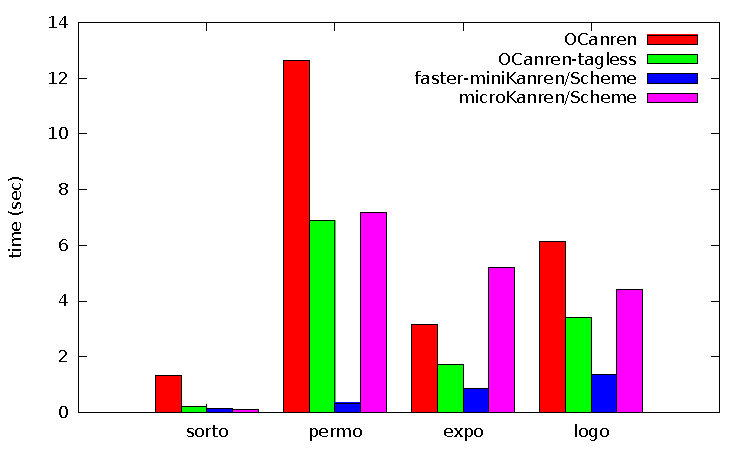
\includegraphics{graph1.pdf}
\caption{The First Set of Benchmarks}
\label{eval:first}
\end{figure}

\begin{figure}[h]
\centering
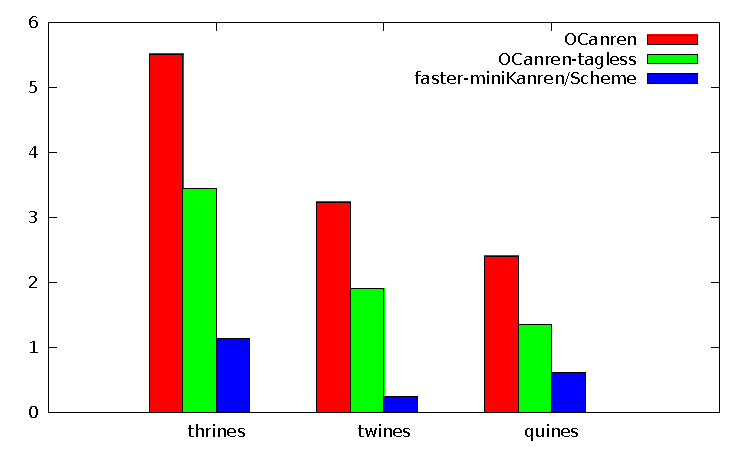
\includegraphics{graph2.pdf}
\caption{The Second Set of Benchmarks}
\label{eval:second}
\end{figure}

\section{Conclusion}

We presented a strongly-typed implementation of \miniKanren for OCaml. Our implementation
passes all tests written for \miniKanren (including those for disequality constraints);
in addition we implemented many interesting relational programs known from
the literature. We claim that our implementation can be used both as a convenient
relational DSL for OCaml and an experimental framework for future research in the area of
relational programming.

%We also want to express our gratitude to William Byrd, who infected us with relational programming,
%and for the extra time he sacrificed as both our tutor and friend.


\begin{acks}
The reported study was funded by RFBR, project number 19-31-90053.
\end{acks}

\bibliographystyle{ACM-Reference-Format}
\bibliography{fair-conj}


\end{document}
\endinput

